\setcounter{part}{1}

\chapter{Contexte}
	\setcounter{chapter}{1}
	\section{SensioLabs}
Créée en 1998 par \emph{Fabien Potencier} et \emph{Grégory Pascal}, \emph{Sensio} est alors une agence digitale basée à Clichy en région parisienne. Renommée \SensioLabs en 2012, la société a aujourd'hui un modèle économique reposant sur la prestation de services, des offres de formation, de conseil et d'accompagnement des déploiements. Ce modèle est en évolution, et \emph{SensioLabs}\footnote{\url{https://sensiolabs.com}} cherche aujourd'hui à s'orienter vers du développement de produits commercialisés en \gls{SaaS}. Ainsi, \emph{SensioLabs Insight}\footnote{\url{https://insight.sensiolabs.com}}, un outil de gestion de qualité des projets \PHP est sorti en 2013, et \emph{Blackfire}\footnote{\url{https://blackfire.io}}, un outil permettant d'analyser les performances de projets \emph{PHP}, est sorti récemment en version commerciale.

\SensioLabs est connu pour son engagement auprès de la communauté open source \PHP grâce au framework \emph{Symfony}\footnote{\url{https://symfony.com}} créé en 2005 par \emph{Fabien Potencier} et utilisé aujourd'hui par de nombreux projets open source, comme Drupal ou phpBB, et entreprises telles que Dailymotion, Yahoo ou Blablacar. Au delà de \emph{Symfony}, \SensioLabs soutient de nombreux projets open source \PHP tels que \emph{Twig}, un moteur de templates très largement utilisé aujourd'hui, \emph{SwitfMailer} ou encore \emph{Silex}.

\clearpage

	\section{Blackfire}

\begin{figure}[!h]
\begin{center}
    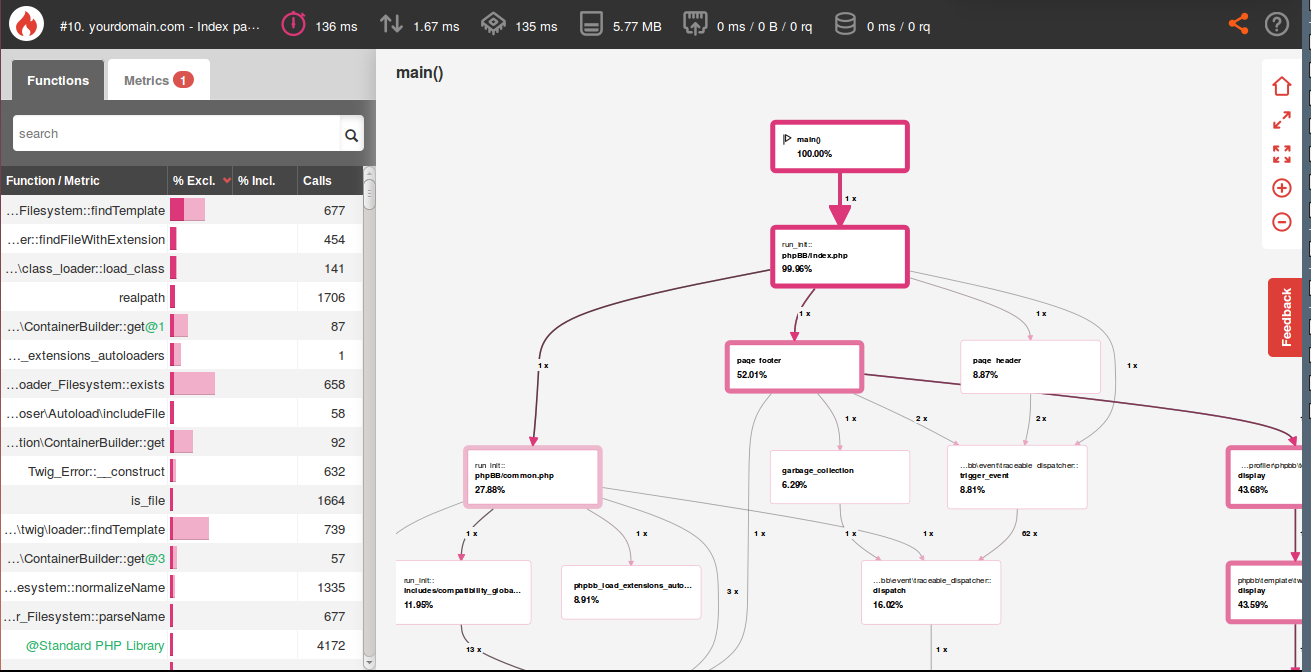
\includegraphics[width=0.8\textwidth]{images/blackfire-exemple}
  %\vspace{-22pt}
  \caption{Exemple de profil généré par \Blackfire}
  \centering
\end{center}
\end{figure}

Dernier outil développé par l'équipe produit de \emph{SensioLabs}, \Blackfire,
sorti commercialement le 27 juillet 2015 après une année de béta test publique, est un produit disponible en mode \gls{SaaS} permettant d'analyser les performances d'applications \PHP de manière simple, précise et juste.

\Blackfire fournit un moyen pour instrumenter automatiquement un code \PHP existant afin d'en extraire des données telles que le \gls{graphe d'appels} du programme ou le temps passé dans chaque fonction, et de les représenter sous une forme graphique intuitive permettant ainsi au développeur d'identifier les principaux problèmes de performance de son application.\footnote{Voir chapitre \vref{chap:Blackfire} pour plus de détails sur \Blackfire et son fonctionnement}

%	\section{Python}
% \Python est un langage de programmation 

\chapter{Objectifs}
	\setcounter{chapter}{2}
	
\begin{figure}[!h]
\begin{center}
  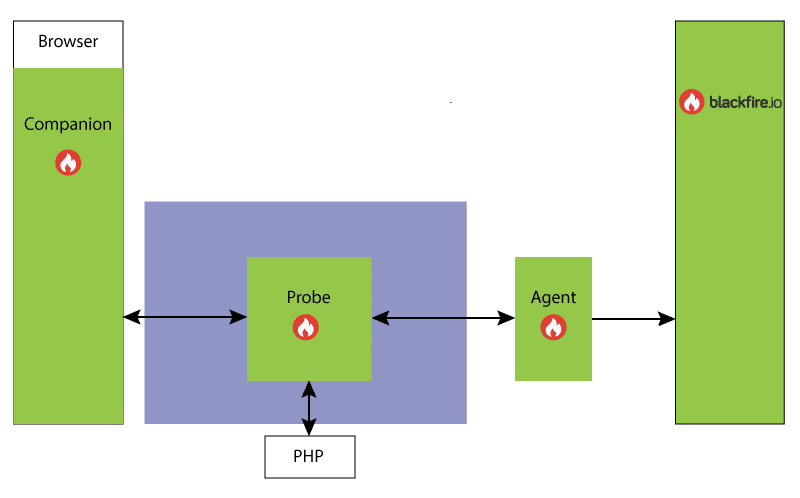
\includegraphics[width=0.8\textwidth]{images/schemas/workflow/archi-general}
  \caption{Organisation générale de \Blackfire}
  % TODO remplacé par le même schéma en simplifié (moins de flèches. le but est de montrer les composants et qui utilise quoi)
\end{center}
\end{figure}

\Blackfire est organisé en quatre composants communiquant les uns avec les autres:
\begin{itemize}
\item Le \textbf{compagnon}, disponible dans \emph{Chrome}, sert à déclencher l'analyse.
\item \textbf{blackfire.io} est le site web qui affiche les résultats.
\item L'\textbf{agent} fait le liens entre la sonde et le site blackfire.io.
\item La \textbf{sonde} est branchée sur le programme de l'utilisateur et collecte des données.
\end{itemize}

Les trois premiers composants ont été conçus de manière à être génériques, et devraient donc être capables de traiter des données issues de n'importe quelle technologie du moment que le protocole\footnote{Voir section \vref{sec:BlackfireProtocol}} est respecté. En pratique il est effectivement possible d'afficher via \textbf{blackfire.io} des profils générés via d'autres outils tel que Callgrind\footnote{\url{http://blog.blackfire.io/cli-upload.html}}, Google Chrome JavaScript CPU profiles\footnote{\url{http://blog.blackfire.io/chrome-cpu-profiles.htmll}} et bien d'autres\footnote{\url{http://blog.blackfire.io/profiling-web-page-loading-performance.html}}\footnote{\url{http://blog.blackfire.io/blackfire-file-format.html}}.

Mais le principal problème d'utiliser ces outils c'est que l'on n'a pas la même expérience que lorsqu'on profile un code \PHP avec \emph{Blackfire}. En effet, lorsqu'on n'utilise pas \Blackfire pour collecter les données on ne peut pas utiliser le compagnon pour déclencher un profil en un clic. De plus l'impact de la collecte des données sur les performances peut être important, et surtout, l'expérience utilisateur peut être compliquée : on peut être obligé d'instrumenter manuellement son code, et une fois le profil généré il faut encore le convertir dans le format utilisé par \Blackfire et l'envoyer sur le site \emph{blackfire.io} à l'aide de la commande \verb|blackfire upload|.

L'enjeu du travail effectué est multiple. Il s'agit d'une part de démontrer que la plate-forme \Blackfire est effectivement générique (et le cas échéant de corriger dans la plate-forme ou le protocole les différents problèmes qui empêchent ou gênent cette généricité), et d'autre part d'apporter le support du langage \emph{Python}.

L'objectif est donc de réaliser une nouvelle implémentation de la quatrième partie, la sonde. Celle-ci serait capable d'analyser des programmes \Python avec une expérience utilisateur la plus proche possible de celle que l'on a actuellement avec la sonde \emph{PHP}. Cela implique que la sonde doit :
\begin{itemize}
  \item permettre d'analyser du code \emph{Python}\footnote{Ceci implique à minima de collecter le graphe d'appels du programme et le temps passé dans chaque fonction/méthode}
  \item communiquer avec l'agent en respectant le protocole
  \item avoir un impact (\gls{overhead}) minimal\footnote{Afin de garantir des résultats aussi fidèles à la réalité que possible}
  \item instrumenter le code automatiquement
  \item ne déclencher l'analyse qu'à la demande\footnote{De cette manière la sonde peut être déployée en production}
\end{itemize}

\setcounter{part}{0}
\setcounter{chapter}{0} 